\chapter{Real-time Web Menggunakan Socket.io}

\section{Apa itu Real-time Web?}

Real-time Web menunjukkan suatu pola interaksi aplikasi Web yang memungkinkan kedua sisi saling mengirimkan data saat terjadi perubahan, jadi tidak seperti pola interaksi yang menghendaki pemakai untuk me-\textit{refresh} browser jika menginginkan data / informasi / \textit{update} terbaru dari sisi server. Contoh dari real-time Web adalah Facebook dan Twitter. Pemakai akan mendapatkan \textit{update} secara langsung saat terjadi perubahan (komentar baru, pesan masuk, permintaan pertemanan, \textit{retweet}, dan lain-lain), tanpa perlu me-\textit{refresh} halaman.

\section{Teknologi Pendukung Real-time Web}

Real-time Web merupakan hal yang relatif kompleks. Terdapat beberapa teknologi yang bisa digunakan untuk mewujudkan real-time Web tersebut. Beberapa diantaranya merupakan standar (atau akan menjadi standar), sedangkan lainnya bukan merupakan standar. 

\subsection{\textit{Ajax Technology}}

Teknologi Ajax (kadang juga ditulis AJAX, singkatan dari \textit{Asynchronous JavaScript and XML} adalah sekumpulan teknologi yang pertama kali dicetuskan oleh Jesse James Garrett. Ajax memungkinkan browser untuk mengirim data dan mengambil data dari server secara \textit{asynchronous} (di latar belakang) tanpa mengganggu keseluruhan tampilan halaman Web. Kumpulan teknologi yang digunakan adalah:
\begin{itemize}
	\item (X)HTML dan CSS untuk presentasi halaman Web
	\item DOM (\textit{Document Object Model}) untuk menampilkan data secara dinamis
	\item XML dan XSLT untuk pertukaran data (seringkali tidak menggunakan XML tetapi JSON).
	\item Obyek XMLHttpRequest untuk komunikasi asynchronous
	\item JavaScript
\end{itemize}

\subsection{Comet dan \textit{Push Technology}}

Comet merupakan istilah payung yang merangkum berbagai teknologi \textit{push}, yaitu teknologi yang memungkinkan server untuk mengirimkan data ke browser tanpa diminta oleh browser.

\subsubsection{SSE (\textit{Server-Sent Events})}

SSE merupakan bagian dari spesifikasi standar HTML5 (bisa diakses di \url{http://dev.w3.org/html5/eventsource/}. Spesifikasi ini memungkinkan server untuk mem-\textit{push} data ke halaman Web menggunakan protokol HTTP. Meski masih dalam pengembangan, tetapi beberapa browser sudah mendukung (misalnya Google Chrome / Chromium) serta Safari. Beberapa peranti pengembangan di sisi server juga sudah mendukung spesifikasi ini. Pada Node.js, pemrogram bisa menggunakan paket sse, nsse, atau EventSource.

\subsubsection{Bayeux Protocol}

Protokol ini dikembangkan oleh \textit{the Dojo Foundation} yang mengembangkan software Dojo Toolkit. Protokol ini digunakan sebagai transport untuk pesan-pesan asynchronous melalui HTTP dengan latensi yang rendah antara klien dengan server. Pesan-pesan tersebut di-rute-kan melalui channel-channel yang diberi nama dan bisa dikirimkan ke:
\begin{itemize}
	\item server ke klien
	\item klien ke server
	\item klien ke klien (melalui server)
\end{itemize}

Spesifikasi lengkap dari protokol ini bisa dilihat di \url{http://svn.cometd.com/trunk/bayeux/bayeux.html}.

\subsubsection{BOSH Protocol}

BOSH (Bidirectional-streams Over Synchronous HTTP) adalah protokol transport yang mengemulasi stream dua arah antara dua entitas (misalnya antara klien dengan server) dengan menggunakan banyak HTTP req/resp yang synchronous tanpa memerlukan polling yang sering atau respon yang terpotong-potong. Spesifikasi ini dikembangkan oleh komunitas serta yayasan XMPP dan bisa dilihat secara lengkap di \url{http://xmpp.org/extensions/xep-0124.html}

\subsection{WebSocket}

WebSocket merupakan teknologi Web yang menyediakan saluran komunikasi full duplex pada satu koneksi TCP. Protokol WebSocket distandarkan oleh IETF di RFC 6455 sedangkap API (\textit{Application Programming Interface}) dikembangkan dan distandarkan oleh W3C sebagai bagian dari HTML5. Komunikasi antara klien dengan server dilaksanakan menggunakan TCP dengan nomor port 80.

WebSocket diimplementasikan di sisi server dan klien dan memungkinkan adanya interaksi yang lebih real-time daripada teknologi push karena protokol dan API ini diimplementasikan dan bisa digunakan di sisi klien maupun server. Browser yang sudah mendukung protokol dan API WebSocket ini adalah Chrome, Firefox, Safari, Opera, dan Internet Explorer. 

Perkembangan dari WebSocket bisa dilihat dan diikuti di \url{http://www.websocket.org/}

\section{Socket.io}

\subsection{Apa itu Socket.io?}

\textit{Socket.io} adalah pustaka JavaScript yang merupakan implementasi dari protokol WebSocket serta berbagai improvisasi lain yang diperlukan untuk real-time web (\textit{heartbeats, timeouts}, dan \textit{disconnection}). Protokol transport yang didukung adalah sebagai berikut:
\begin{itemize}
\item WebSocket
\item Adobe Flash Socket
\item AJAX long polling
\item AJAX multipart streaming
\item Forever Iframe
\item JSONP Polling
\end{itemize}
Pustaka ini terdiri atas pustaka untuk sisi klien (browser) dan server (menggunakan Node.js). Browser yang didukung adalah:
\begin{itemize}
\item Internet Explorer 5.5+ (desktop)
\item Safari 3+ (desktop)
\item Google Chrome 4+ (desktop)
\item Firefox 3+ (desktop)
\item Opera 10.61+ (desktop)
\item iPhone Safari (mobile)
\item iPad Safari (mobile)
\item Android WebKit (mobile)
\item WebOs WebKit (mobile)
\end{itemize}

\subsection{Menggunakan Socket.io untuk Real-time Web}

Socket.io melibatkan sisi klien dan sisi server. Pada sisi server, paket yang diperlukan adalah cocket.io, sementara untuk sisi klien (browser), diperlukan socket.io-client. Paket socket.io-client tidak diperlukan langsung pada sisi node\_modules, tetapi ada beberapa file yang harus ditempatkan pada akses publik dengan maksud supaya bisa digunakan oleh browser. 

\subsubsection{Tentang Aplikasi}

Aplikasi ini hanya merupakan contoh kecil dari real-time Web. Aplikasi terdiri atas sisi server dan klien/browser. Pada sisi server, aplikasi ini akan mengirimkan data ke browser (push). Sementara itu, browser akan menerima hasil push tersebut dan menampilkannya kemudian mengirimkan data ke server tanpa perlu melakukan proses \textit{refresh}. Server hanya akan menampilkan data yang dikirimkan browser. 

\subsubsection{Membuat Kerangka Aplikasi dengan ExpressJS}

Untuk membuat aplikasi ini, kita akan menggunakan ExpressJS dan Socket.io. Pada awalnya, kita akan membuat kerangka aplikasi menggunakan express (jika ExpressJS belum terinstall, install dengan menggunakan \textit{npm install -g express}. 

\lstset{language=Bash,caption=Membuat kerangka aplikasi dengan ExpressJS}
\begin{lstlisting}
$ express 

   create : .
   create : ./package.json
   create : ./app.js
   create : ./public
   create : ./public/images
   create : ./public/stylesheets
   create : ./public/stylesheets/style.css
   create : ./routes
   create : ./routes/index.js
   create : ./routes/user.js
   create : ./views
   create : ./views/layout.jade
   create : ./views/index.jade
   create : ./public/javascripts

   install dependencies:
     $ cd . && npm install

   run the app:
     $ node app
\end{lstlisting}

Pada pembahasan berikutnya, kita akan mengadakan berbagai perubahan yang diperlukan.

\subsubsection{Instalasi Paket yang Diperlukan}

File \textit{package.json} berisi beberapa informasi tentang aplikasi ini serta beberapa paket yang diperlukan. Isi dari file ini adalah sebagai berikut:

\lstset{language=JavaScript,caption=package.json}
\begin{lstlisting}
{
  "name": "socket.io-expressjs",
  "version": "0.0.1",
  "author": "Bambang Purnomosidi D. P.",
  "private": true,
  "scripts": {
    "start": "node app"
  },
  "dependencies": {
    "express": "latest",
    "jade": "*",
    "socket.io": "latest",
    "socket.io-client": "latest"
  }
}
\end{lstlisting}

Setelah itu. install paket-paket tersebut dengan menggunakan perintah \textit{npm install} di direktori tersebut. 

\subsubsection{Konfigurasi JavaScript untuk Browser}

Browser juga memerlukan pustaka untuk Socket.io yang diperoleh dari paket \textit{socket.io-client}. Pada paket tersebut, terdapat direktori \textit{dist}:

\lstset{language=Bash,caption=Isi direktori dist di socket.io-client}
\begin{lstlisting}
$ ls node_modules/socket.io-client/dist/
total 496
drwxr-xr-x 2 bpdp users   4096 Dec 16 20:18 .
drwxr-xr-x 7 bpdp users   4096 Dec 16 20:18 ..
-rw-r--r-- 1 bpdp users 101222 Nov  2 22:02 socket.io.js
-rw-r--r-- 1 bpdp users  44789 Nov  2 22:02 socket.io.min.js
-rw-r--r-- 1 bpdp users 175953 Mar 28  2012 WebSocketMainInsecure.swf
-rw-r--r-- 1 bpdp users 175830 Mar 28  2012 WebSocketMain.swf
\end{lstlisting}

\textit{Copy}-kan file-file tersebut ke direktori \textit{public/javascripts}.

\subsubsection{Hapus File yang Tidak Diperlukan}

Ada beberapa file yang tidak diperlukan dan harus dihapus:
\begin{itemize}
	\item routes/user.js
\end{itemize}

\subsubsection{Ubah File-file Tertentu}

Beberapa file akan diedit. Beberapa diantaranya akan diuraikan di bagian ini.

\lstset{language=JavaScript,caption=app.js}
\begin{lstlisting}
var express = require('express')
		, app = express()
  	, routes = require('./routes')
	  , http = require('http')
		, server = http.createServer(app)
	  , io = require('socket.io').listen(server);

server.listen(80);

app.configure(function(){
  app.set('views', __dirname + '/views');
  app.set('view engine', 'jade');
  app.use(express.favicon());
  app.use(express.logger('dev'));
  app.use(express.bodyParser());
  app.use(express.methodOverride());
	app.use(express.static(__dirname + '/public'));
  app.use(app.router);
});

app.get('/', routes.index);

io.sockets.on('connection', function (socket) {
	socket.emit('kirim ke browser', { 
		kalimatDariServer: 'Kalimat ini dikirim dari server' });
	socket.on('dari browser', function (data) {
		console.log(data.kalimatDariBrowser);
	});
});
\end{lstlisting}

\lstset{language=html,caption=views/index.jade}
\begin{lstlisting}
extends layout

block content
  h1= title
  p #{title}
  script(src="/javascripts/socket.io.js")
  script
    var socket = io.connect('http://localhost');
    socket.on('kirim ke browser', function (data) {
      document.getElementById("container").innerHTML=
        "<p>" + data.kalimatDariServer + "</p>";
      socket.emit('dari browser', { 
        kalimatDariBrowser: 'Kalimat ini dikirim dari browser' });
    });
  #container
    p #{title}
\end{lstlisting}

\lstset{language=html,caption=routes/index.js}
\begin{lstlisting}
/*
 * GET home page.
 */

exports.index = function(req, res){
  res.render('index', { title: 'Contoh Socket.io + Express' });
};
\end{lstlisting}

\subsubsection{Menjalankan Server Socket.io}

Server socket.io menggunakan port 80 sehingga harus dijalankan oleh \textit{root}. 

\lstset{language=Bash,caption=Menjalankan server Socket.io}
\begin{lstlisting}
# node app.js 
   info  - socket.io started
   debug - client authorized
   info  - handshake authorized qrMUlAcSRMywnvUK31RV
   debug - setting request GET /socket.io/1/websocket/qrMUlAcSRMywnvUK31RV
   debug - set heartbeat interval for client qrMUlAcSRMywnvUK31RV
   debug - client authorized for 
   debug - websocket writing 1::
   debug - websocket writing 5:::{"name":"kirim ke browser","args":[{"kalimatDariServer":"Kalimat ini dikirim dari server"}]}
Kalimat ini dikirim dari browser
GET / 200 44ms - 628
   info  - transport end (socket end)
   debug - set close timeout for client qrMUlAcSRMywnvUK31RV
   debug - cleared close timeout for client qrMUlAcSRMywnvUK31RV
   debug - cleared heartbeat interval for client qrMUlAcSRMywnvUK31RV
   debug - discarding transport
GET /javascripts/socket.io.js 304 4ms
GET /stylesheets/style.css 304 4ms
   debug - client authorized
   info  - handshake authorized Eug556Y-X-4R8fOB31RW
   debug - setting request GET /socket.io/1/websocket/Eug556Y-X-4R8fOB31RW
   debug - set heartbeat interval for client Eug556Y-X-4R8fOB31RW
   debug - client authorized for 
   debug - websocket writing 1::
   debug - websocket writing 5:::{"name":"kirim ke browser","args":[{"kalimatDariServer":"Kalimat ini dikirim dari server"}]}
Kalimat ini dikirim dari browser
   debug - emitting heartbeat for client Eug556Y-X-4R8fOB31RW
   debug - websocket writing 2::
   debug - set heartbeat timeout for client Eug556Y-X-4R8fOB31RW
   debug - got heartbeat packet
   debug - cleared heartbeat timeout for client Eug556Y-X-4R8fOB31RW
   debug - set heartbeat interval for client Eug556Y-X-4R8fOB31RW
	 ...
	 ...
	 ...
	 ...
\end{lstlisting}

Keluaran pada sisi server tersebut merupakan keluaran yang sudah termasuk akses dari browser. Setelah server dijalankan, buka browser kemudian akses URL \url{http://localhost}. Setelah diakses melalui browser, server akan mengirimkan kode sumber HTML sebagai berikut:

\lstset{language=html,caption=Kode sumber di browser}
\begin{lstlisting}
<!DOCTYPE html>
<html>
	<head>
		<title>Contoh Socket.io + Express</title>
		<link rel="stylesheet" href="/stylesheets/style.css">
	</head>
	<body>
		<h1>Contoh Socket.io + Express</h1>
		<p>Contoh Socket.io + Express</p>
		<script src="/javascripts/socket.io.js"></script>
		<script>
			var socket = io.connect('http://localhost');
			socket.on('kirim ke browser', function (data) {
			  document.getElementById("container").innerHTML=
			    "<p>" + data.kalimatDariServer + "</p>";
			socket.emit('dari browser', { 
		    kalimatDariBrowser: 'Kalimat ini dikirim dari browser' });
			});
		</script>
		<div id="container">
			<p>Contoh Socket.io + Express</p>
		</div>
	</body>
</html>
\end{lstlisting}

Tampilan di browser bisa dilihat pada gambar~\ref{fig:socket-io-express}

  \begin{figure}
    \begin{center}
      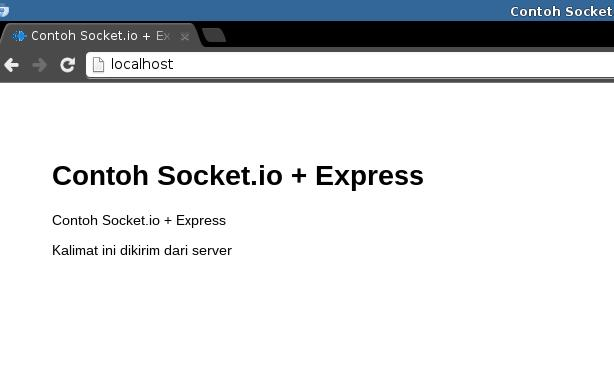
\includegraphics[scale=0.5]{images/socket-io-expressjs.jpg}
    \end{center}
    \caption{Hasil di browser dari ExpressJS + Socket.io}
    \label{fig:socket-io-express}
  \end{figure}

Contoh pada materi ini merupakan contoh sederhana, tetapi diharapkan bisa dengan mudah dipahami untuk membuat aplikasi Web real-time. 
